\newpage
\subsection{Планирование сырья}
\label{bp:RawMaterialPlanning}

\textbf{Планирование бумаги и картона}

Планирование основного сырья (бумага и картон) выполняет специалист отдела снабжения.
На гофроагрегате при использовании сырья разработан нормативный документ по возможным заменам сырья. 
Планирование сырья выполняется в конце месяца на будущий месяц.

Специалист отдела снабжения ведет таблицу в Excel (форма \ref{pic:d35}) по планированию сырья.
Для планирования сырья специалист отдела снабжения получает остатки из системы 1С:УПП по форме \ref{pic:d36}.
Товары в пути определяет по данным своего файла форма \ref{pic:d35} вручную.
Специалист отдела снабжения определяет расчетным путем остаток сырья в месяцах работы оборудования.
План закупки специалист отдела снабжения считает вручную в форме \ref{pic:d37}.
Далее специалист отдела снабжения распределяет потребности в сырье по поставщикам. Cпециалист отдела снабжения создает запрос у поставщиков по цене и объемам поставки на каждый месяц.

Специалист отдела снабжения создает вручную заявку на поставку по форме \ref{pic:d38}.

Потребности в краске определяет отдел ОТК (отдел подготовки производства).
Заказывает краску специалист отдела снабжения.
В системе 1С:УПП специалист отдела снабжения смотрит только приход материалов.



% \textbf{Планирование закупки заготовок}

% На производстве выделены популярные позиции заготовок, по которым имеется складской запас. 


% По таким изделиям МСЗ контролируют объем неснижаемого запаса вручную и при необходимости создают заказы покупателя на контрагента ООО ''Рускартон'' (на склад). 
% Остальные заготовки поступают сразу в производство под конкретный производственный заказ.
% МСЗ на основании заказа покупателя создает заказ на бронь по складским свободным остаткам. Остатки МСЗ может узнать по отчету в 1С:УНФ «Остатки ГП». В момент отгрузки менеджер снимает с резерва свободные остатки в разрезе заказа покупателя.

% Планированием закупки заготовок занимается инженер по планированию.
% Заказ от менеджера поступает в системе 1С:УНФ инженеру по планированию, который на основании плана производства в таблице MS Excel (рис. ??) создает в системе 1С:УНФ документ ''Заявка на продажу'' (рис. \ref{pic:d17}). 

% % \todo{перечитать с планированием}

% При создании заказа менеджеры стараются создавать заказ на производство кратно поддону. 
% Инженер по планированию ставит в системе 1С:УНФ у документа ''Заказ на производство'' статус «В работе» и заказывает заготовки у поставщиков согласно заказам на производство. Объем заказа заготовок в точности совпадает с объемом заказа на производство.
% На основании формы \ref{pic:d15} инженер по планированию формирует заявку на производство (заготовки) и заявку на ресурсе поставщика.

\textbf{Планирование вспомогательных материалов}

Планированием и закупкой вспомогательных материалов занимается отдел снабжения.

% Каждый день техник по учету определяет остатки по крахмалу и другим материалам (Пленка, скотч и др.) в производстве и сообщает по телефону в отдел снабжения остатки на складе. 25 числа каждого месяца менеджер по снабжению заказывает поставки крахмала на следующий месяц. Объемы заказа определяются коллективно с техником по учету. Менеджер отдела снабжения обзванивает поставщиков по ценам, формирует заявку в свободной форме. Поставки крахмала выполняются 2-3 раза в месяц.

В системе 1С:УПП хранятся текущие остатки на складах.


По закупке других материалов (СИЗ, спецодежда, комплектующие и запчасти) отдел снабжения собирает заявки от подразделений, обрабатывает их, ищет поставщиков и производит закупку.


\textbf{Поддоны}

Учет поддонов осуществляется в Файле MS Excel, который ведет главный технолог. Но заказ поддонов производят начальники смен. Начальники смен определяют потребность в поддонах исходя из плана производства и текущих остатков на складах и  сообщают в отдел снабжения. Отдел снабжения производит закупку необходимого количества поддонов.  
% Начальник склада каждый вечер определяет потребность по поддонам и сообщает по телефону в отдел снабжения, где менеджеры отдела снабжения фиксирует вручную объемы потребности.
% Коммерческий отдел и отдел снабжения совместно определяют потребность в поддонах исходя из плана производства и текущих остатков на складах и заказывают поддоны у производителей.
% Менеджеры отдела снабжения создают заявку на закупку поддонов и спецподдонов. Все поддоны невозвратные.
% Поддоны принимаются на складе. Учет поступления фиксируется в системе СБИС.


\textbf{Планирование краски}

На предприятии используют готовую краску. Учет краски возложен на контролеров по качеству (технологов). Остатки  краски технолог определяет визуально и сообщает специалисту отдела снабжения позиции, которые необходимо приобрести. Отчеты по расходу ведутся в MS Excel и контролируются главным технологом  \ref{pic:1.9 отчет о расходе сырья и материалов 2_0001}.
%\todo{ПИСАТЬ}
% Краску заказывает техник УВФ (???). Остатки основы и пигментов краски техник определяет визуально и по опыту заказывает необходимый объем напрямую у поставщика.



%Оснастку тоже.

% Закупками краски занимается инженер по планированию. Краска в цеху списывается ежедневно. Инженер по планированию ориентируясь на недельный план в таблице MS Excel, составляет потребность в краске на неделю и сравнивает с остатками в 1С (рис. \ref{pic:a80}). При наличии нужного пантона менее 20 кг (1 ведра), заказывается еще 20 кг.

% \begin{figure}
% \begin{center}
%   \includegraphics[height=0.6\textheight, keepaspectratio]{Pics/a80.jpg}
% \end{center}
%   \caption{Остатки по краске}
%   \label{pic:a80}
% \end{figure}
% \clearpage

% \textbf{Планирование вспомогательных материалов }

% Вспомогательные материалы закупает инженер по планированию. Списание на производстве происходит в конце месяца. По просьбе инженера по планированию кладовщик может пересчитать и предоставить остатки на бумаге (\ref{pic:a57}). Ориентируясь на них инженер по планированию закупает необходимые материалы. Клей закупает на месяц 240 кг (1 бочка).

% Мастер производства заказывает поддоны  по телефону, контролирует остатки  и заказывает недостающее количество. Перемещение поддонов выполняет  бухгалтер по накладной (\ref{pic:a31}). Поддоны от поставщиков (приходит заготовка) сразу увозят на другую площадку для сортировки. 

\begin{figure}
\begin{center}
  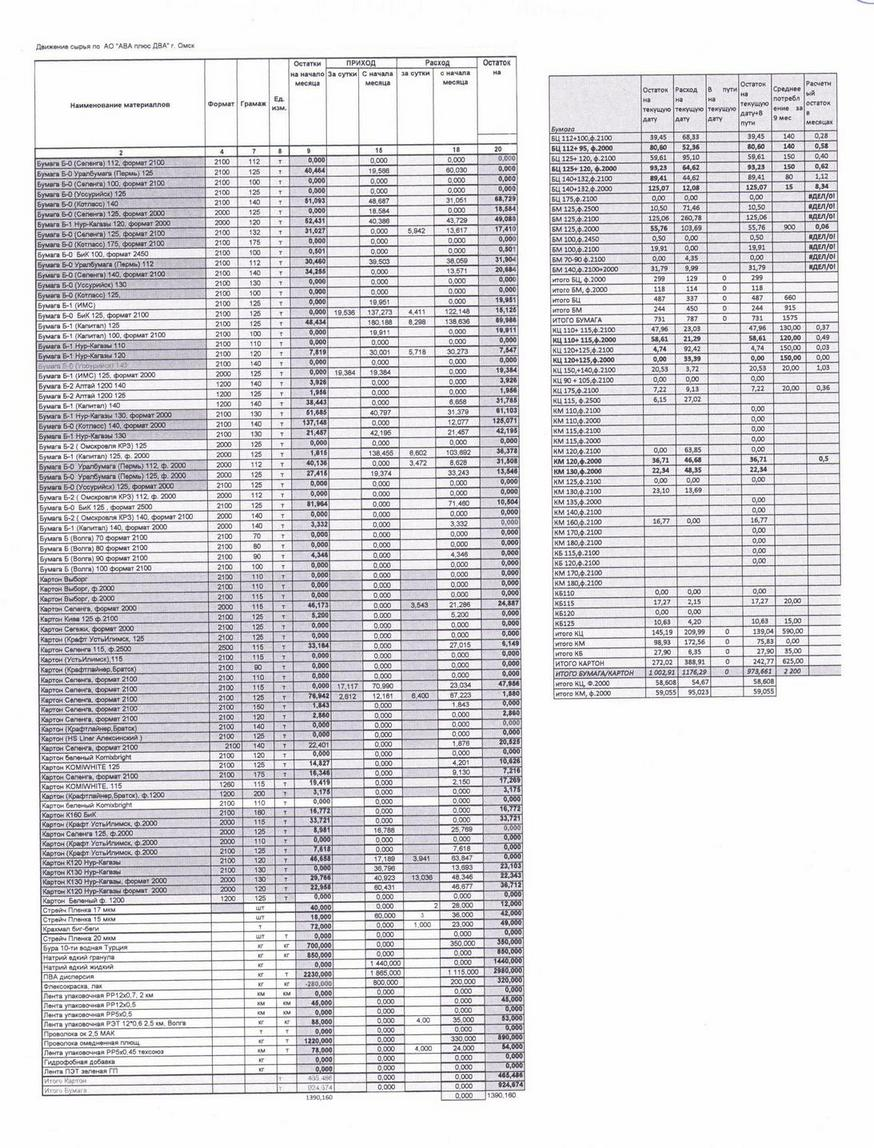
\includegraphics[height=0.9\textheight, keepaspectratio]{Pics/d35.jpg}
\end{center}
  \caption{Форма планирования сырья}
  \label{pic:d35}
\end{figure}
\clearpage

\begin{figure}
\begin{center}
  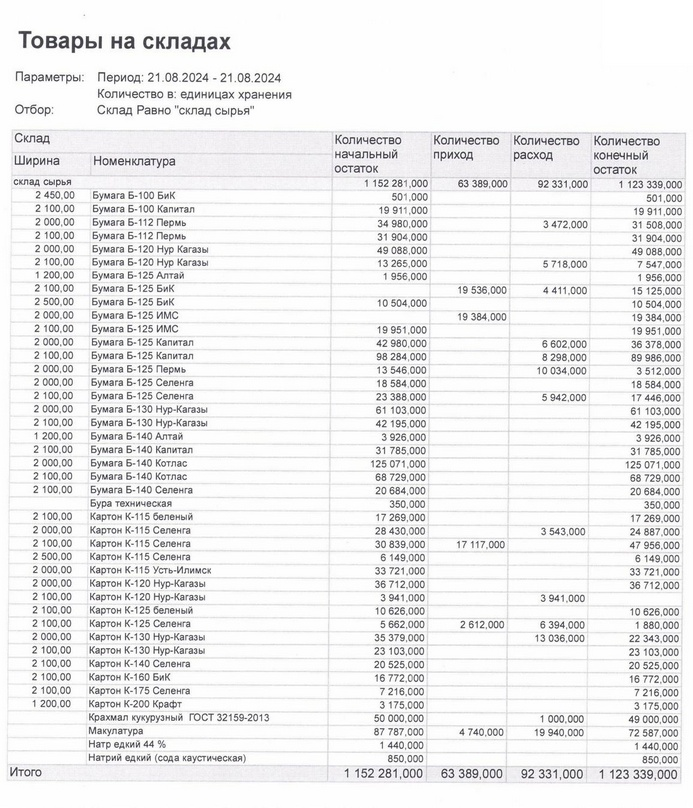
\includegraphics[height=0.8\textheight, keepaspectratio]{Pics/d36.jpg}
\end{center}
  \caption{Форма остатков из системы 1С:УПП по бумаге и картону}
  \label{pic:d36}
\end{figure}
\clearpage

\begin{figure}
\begin{center}
  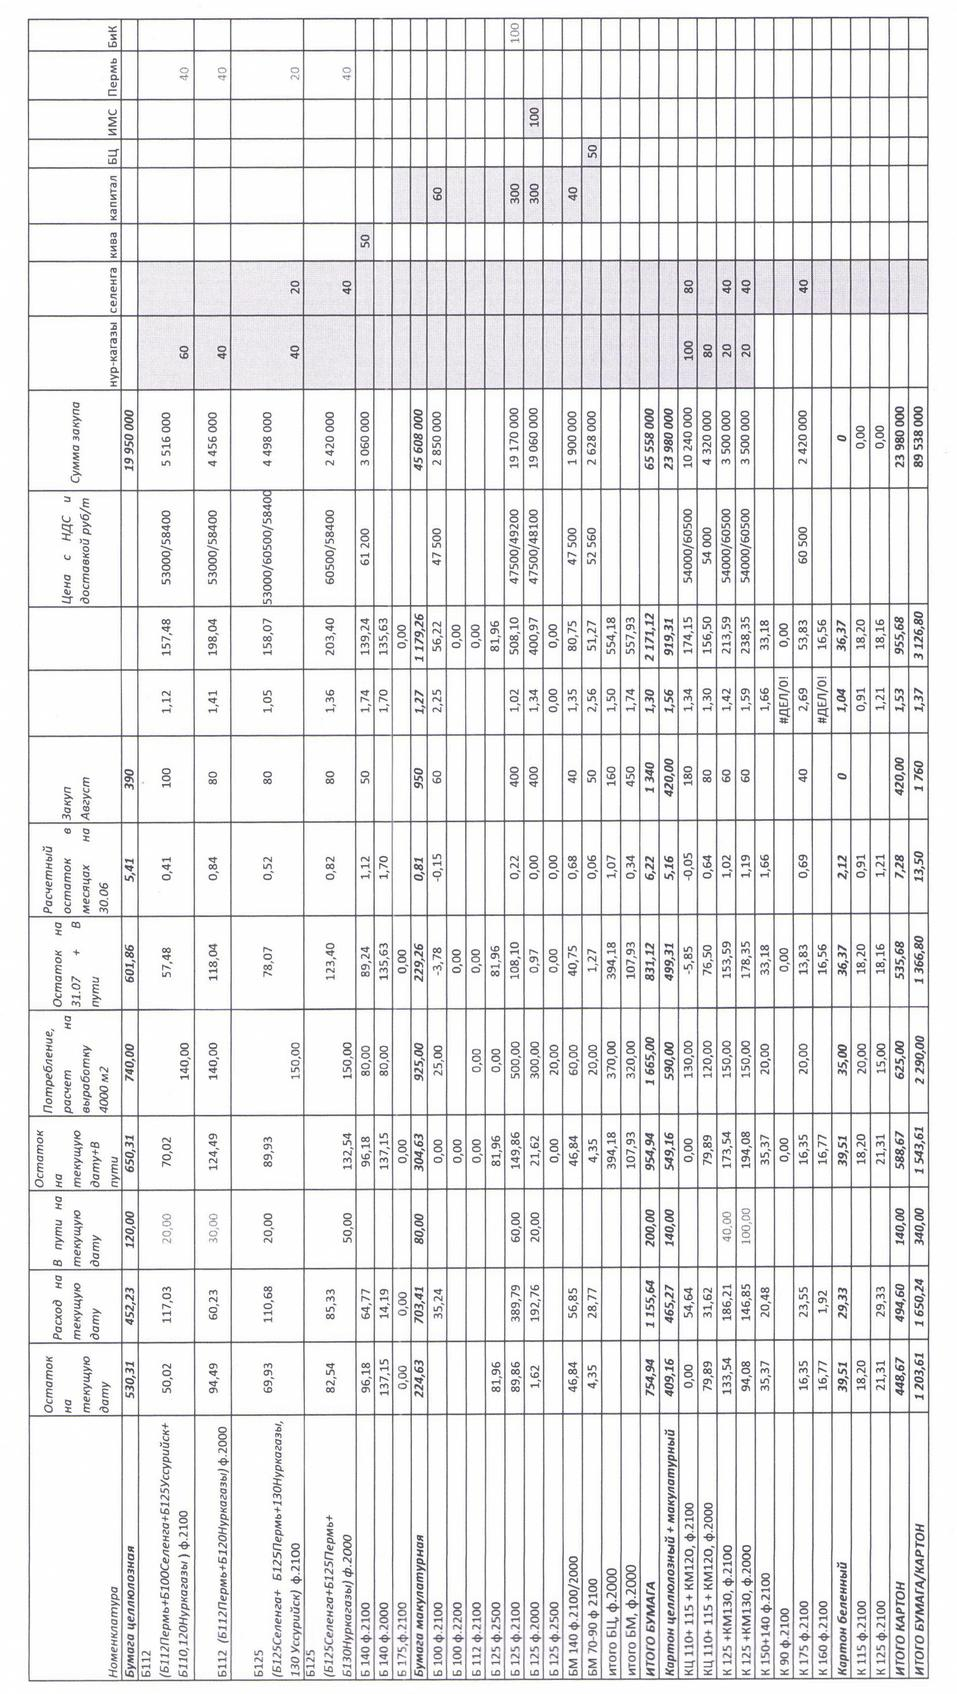
\includegraphics[height=0.8\textheight, keepaspectratio]{Pics/d37.jpg}
\end{center}
  \caption{Форма расчета потребности в сырье}
  \label{pic:d37}
\end{figure}
\clearpage

\begin{figure}
\begin{center}
  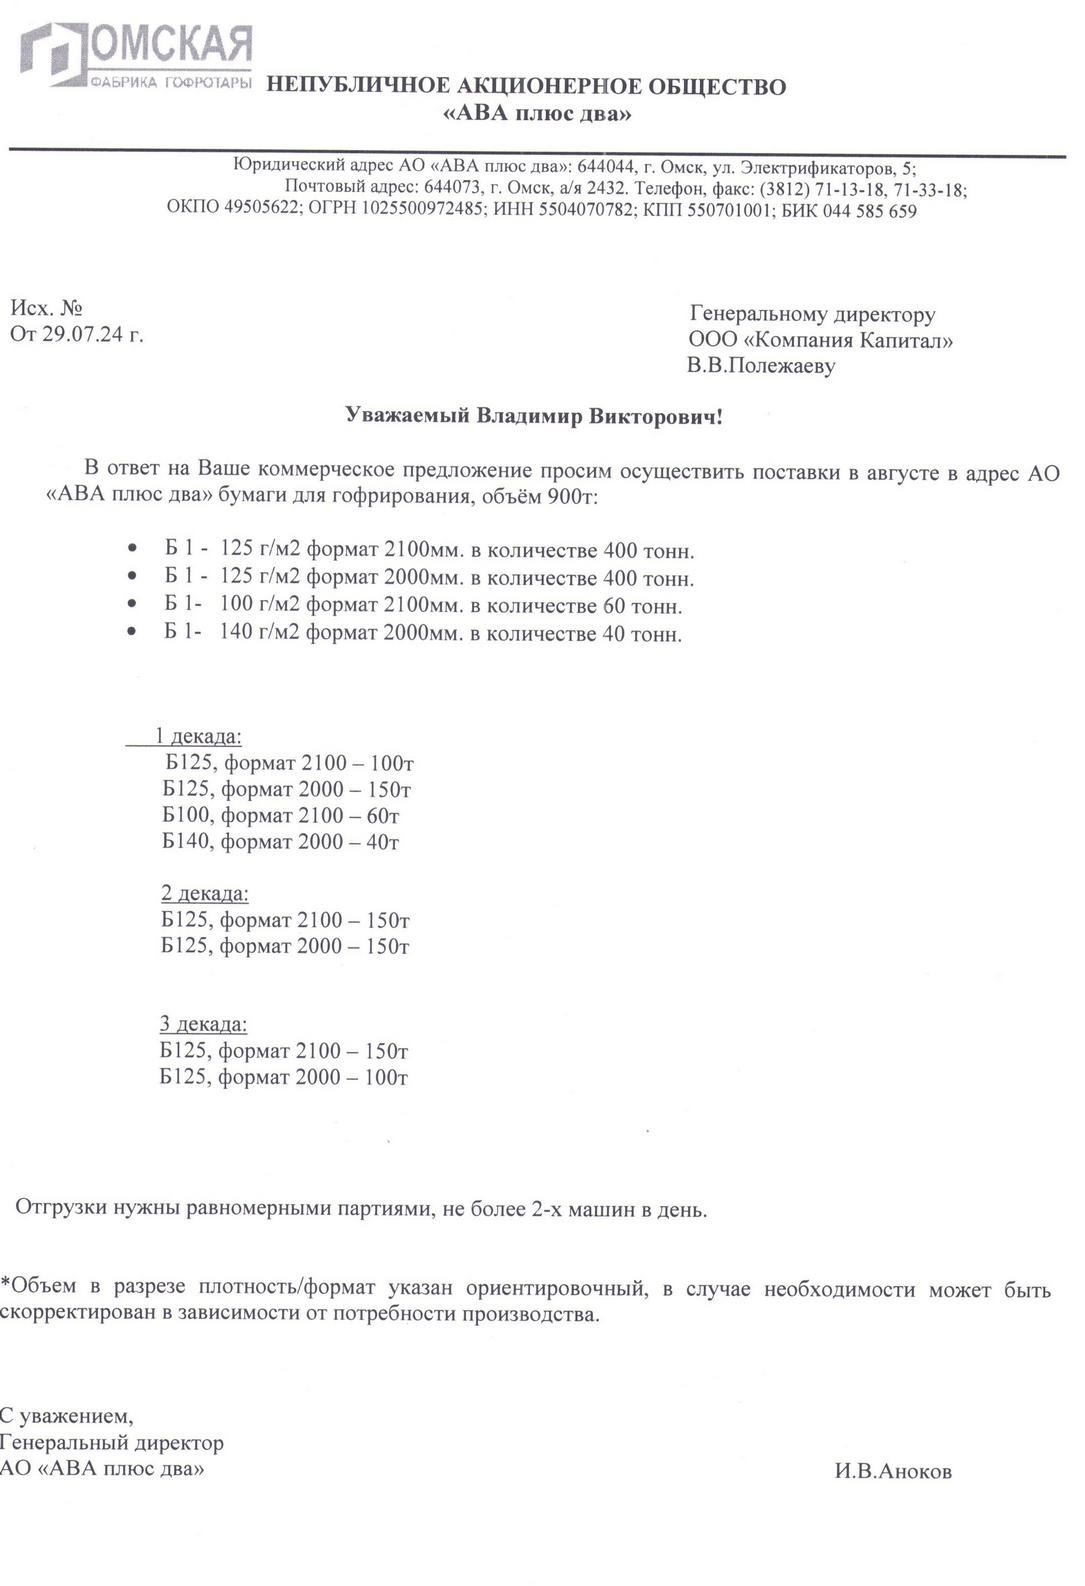
\includegraphics[height=0.8\textheight, keepaspectratio]{Pics/d38.jpg}
\end{center}
  \caption{Форма заявки на поставку сырья}
  \label{pic:d38}
\end{figure}
\clearpage

\begin{figure}
\begin{center}
  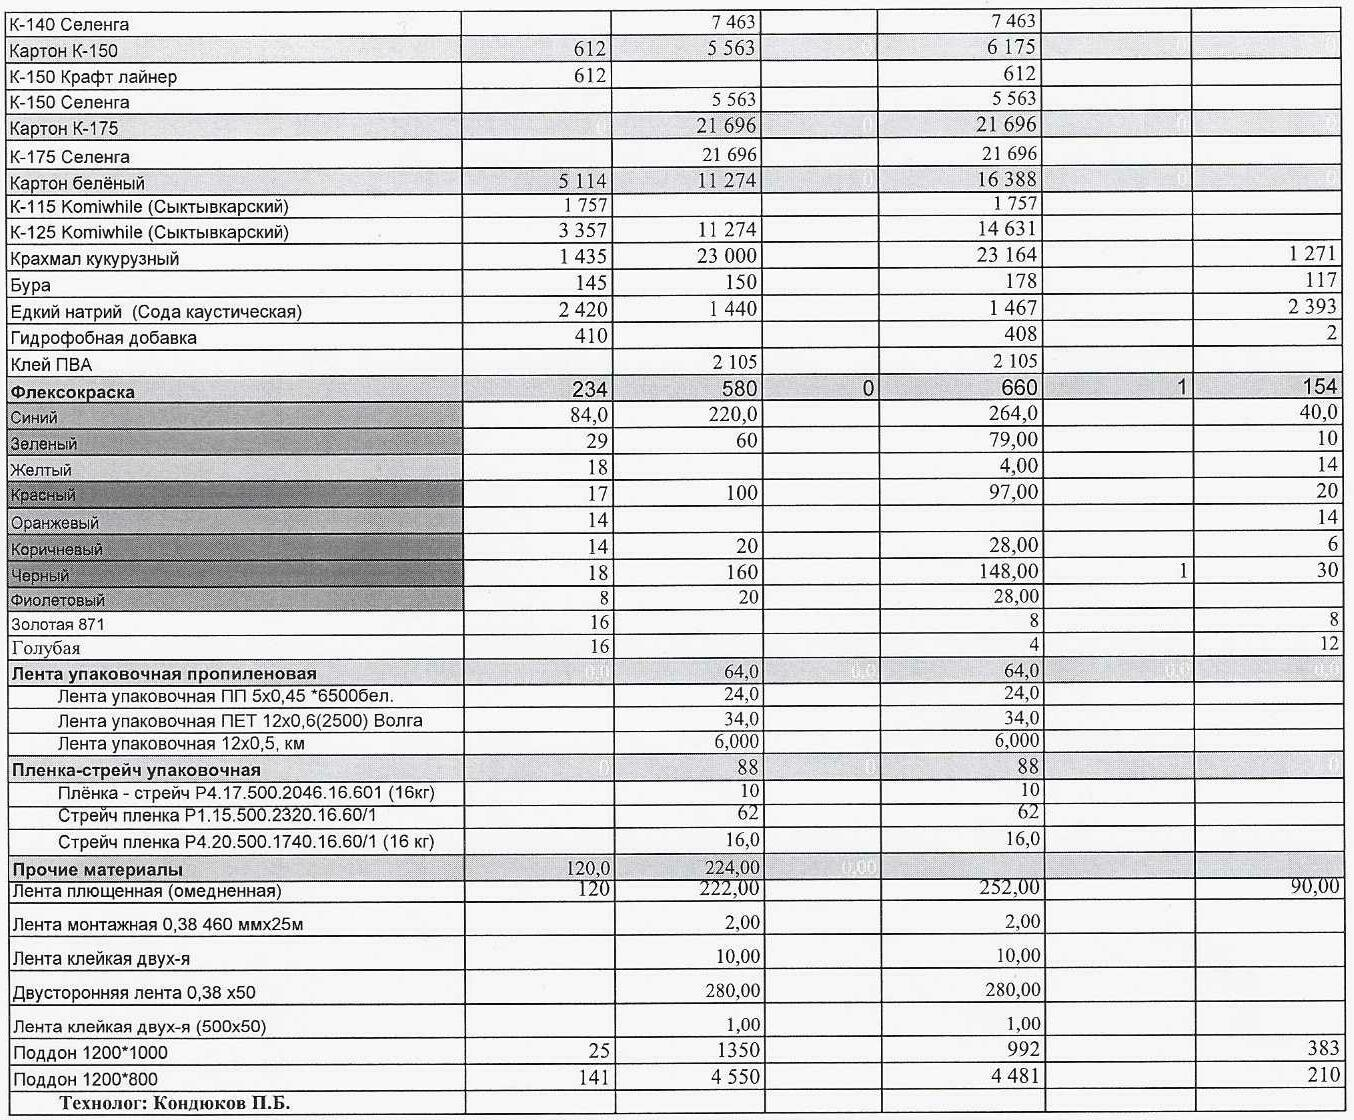
\includegraphics[height=0.6\textheight, angle=90, keepaspectratio]{Pics 1/1.9 отчет о расходе сырья и материалов 2_0001.jpg}
\end{center}
  \caption{Учет сырья и материалов в MS Excel}
  \label{pic:1.9 отчет о расходе сырья и материалов 2_0001}
\end{figure}
\clearpage
%
\clearpage
\ifx \notincludehead\undefined
\normalsize
\end{document}
\fi